
%(BEGIN_QUESTION)
% Copyright 2009, Tony R. Kuphaldt, released under the Creative Commons Attribution License (v 1.0)
% This means you may do almost anything with this work of mine, so long as you give me proper credit

Calculate the percentage of incident power reflected back to the transmitter, and the percentage of incident power transmitted (forward) through the liquid in this radar level measurement application:

$$\includegraphics[width=15.5cm]{i04217x01.eps}$$

Also, calculate the ullage and fillage for this vessel, given a reflected pulse (``echo'') time of 18.3 nanoseconds and a total vessel height of 30 feet.

\vskip 20pt \vbox{\hrule \hbox{\strut \vrule{} {\bf Suggestions for Socratic discussion} \vrule} \hrule}

\begin{itemize}
\item{} Suppose the permittivity of the vapor were to increase.  How would this affect the calibration of the radar transmitter?  Would it result in a zero shift, a span shift, a change in linearity, or some combination of these?
\item{} Identify different process conditions that would result in the permittivity of the vapor significantly changing.
\end{itemize}


\underbar{file i04217}
%(END_QUESTION)





%(BEGIN_ANSWER)

$P_{reflected}$ = 26.15\%

\vskip 10pt

$P_{forward}$ = 73.85\%

\vskip 10pt

Ullage = 8 feet 4.7 inches

\vskip 10pt

Fillage = 21 feet 7.3 inches

\vskip 10pt

(Note: the velocity of light used in the ullage and fillage calculations is $2.9979 \times 10^8$ meters per second)

\vskip 10pt

The 35 PSI gas pressure is extraneous information, included for the purpose of challenging students to identify whether or not information is relevant to solving a particular problem.  Gas pressure is relevant for a radar level instrument only because changes in gas pressure can cause the gas permittivity to change as well, thus influencing the radio wave's propagation velocity.  However, since we are already given the permittivity value of the gas in this situation, the pressure is irrelevant.

%(END_ANSWER)





%(BEGIN_NOTES)

Reflection factor:

$$R = {\left({\sqrt{\epsilon_{r2}} - \sqrt{\epsilon_{r1}}}\right)^2 \over \left(\sqrt{\epsilon_{r2}} + \sqrt{\epsilon_{r1}}\right)^2}$$

$$R = {\left({\sqrt{11} - \sqrt{1.15}}\right)^2 \over \left(\sqrt{11} + \sqrt{1.15}\right)^2} = 0.26146$$

If 26.146\% of the power gets reflected by the vapor/liquid interface, the remaining power (73.854\%) must pass through the interface.

\vskip 10pt

Velocity of propagation through the gas:

$$v = {c \over \sqrt{\epsilon_r}}$$

$$v = {2.9979 \times 10^8 \hbox{ m/s} \over \sqrt{1.15}} = 2.79556 \times 10^8 \hbox{ m/s}$$

\vskip 10pt

Ullage calculation:

$$x = vt$$

$$\hbox{Ullage} = 0.5 x = 0.5 vt$$

$$\hbox{Ullage} = (0.5) (2.79556 \times 10^8 \hbox{ m/s}) (18.3 \hbox{ ns})$$

$$\hbox{Ullage} = 2.5579 \hbox{ m} = 8.392 \hbox{ ft} = 8 \hbox{ ft } 4.7 \hbox{ in}$$

\vskip 10pt

Fillage calculation:

$$\hbox{Fillage} = \hbox{Total height} - \hbox{Ullage}$$

$$\hbox{Fillage} = 30 \hbox{ ft} - 8.392 \hbox{ ft}$$

$$\hbox{Fillage} = 21.61 \hbox{ ft} = 21 \hbox{ ft } 7.3 \hbox{ in}$$

%INDEX% Measurement, level: radar

%(END_NOTES)


